\documentclass[10pt]{article}
\usepackage{amsmath,amssymb,amsthm,booktabs,array}
\usepackage[hidelinks]{hyperref}
\usepackage{tikz,placeins}
\usepackage{flafter,needspace}
\renewcommand{\topfraction}{.9}
\renewcommand{\bottomfraction}{.85}
\renewcommand{\textfraction}{.08}
\renewcommand{\floatpagefraction}{.8}
\setcounter{topnumber}{5}
\setcounter{totalnumber}{6}
\AddToHook{cmd/section/before}{\Needspace{6\baselineskip}}
\usetikzlibrary{arrows.meta,positioning}
\usepackage{style/hkustgz-paper}
\newtheorem{proposition}{Proposition}
\newcommand{\D}{\mathcal D}
\newcommand{\W}{\mathcal W}
\title{When Battery-Free Interfaces Support Design Changes\\Qualified Observations and Strong Static Controls}
\hypersetup{pdftitle={When Battery-Free Interfaces Support Design Changes: Qualified Observations and Strong Static Controls},pdfauthor={Development manuscript}}
\author{Development manuscript}
\papersubtitle{20 October 2026}
\date{20 October 2026}
\begin{document}
\maketitle
\begin{abstract}
Battery-free design decisions depend on when energy is usable, which event
state survives reset, and what reaches the receiver. Current success can omit
the mechanism activated by a legal design change. We distinguish current-verdict
from intervention sufficiency, give an elementary factorization condition, and
connect storage and reset counterexamples to a source-bound observation
interface. An earlier four-task comparison gives 8/12 service passes with
average-energy inputs and 12/12 with each strong static or executable control;
live observation completes seven chains and leaves five incomplete. We retain
these failures and add deterministic cross-source unit, domain and type
preflight before actual consumption. A new frozen comparison uses storage
connection, reset placement and package-response interventions, each in two
fresh contexts per arm. Complete information, conservative fixed rules and
observation refinement each produce 6/6 correct predictions, decisions and
selected-service passes. Typed observation consumption occurs in 1/6, 4/6 and
3/6 respectively; it is a path statistic, not the success criterion for direct
baselines. Two fixed-rule episodes stop at the request cap after correct
submissions. Refinement uses 50 requests versus complete information's 37,
with equal source acquisition and a slightly lower fixed-rate fee estimate:
there is no accuracy, acquisition or comprehensive cost advantage. Saved event
studies additionally separate matched delivery from encoded-time accuracy.
All results concern prescribed-source digital apparatus; physical qualification
is unavailable and the original product remains unaccepted.
\end{abstract}
\section{Introduction}
A battery-free device must turn an intermittent supply into a particular
service: capture an external event, preserve the relevant state, and deliver
the required information at the required time. A source integral does not
specify when a rail becomes ready, whether a transmit pulse causes a reset,
or whether the pending event is still present when power returns. Intermittent
execution mechanisms and type systems address parts of this consistency
problem~\cite{alpaca,curricle}. The design consumer also needs an interface
that exposes the laws and state transitions affected by its next legal change.

The information requirement is prospective. Two worlds can have identical
current traces yet different unexcited storage clamps; reducing capacitance
then separates their outcomes. Two event memories can likewise agree until a
reset occurs. These witnesses explain why a current successful trace need not
support intervention. They do not establish a universal advantage for live
observations: a static description containing the relevant laws, parameters,
initial state and intervention domain can already determine the answer.
Our elementary distinguishability condition states that boundary without
claiming a new general abstraction theory~\cite{cegar,structural,mechanisms}.

An observation interface provides an operational route from information to
action. It acquires a source, selects or constructs a relation, checks its
domain and units, and delivers a typed value to a design policy. Each step can
fail independently. An equation can refer to the wrong source-local domain;
a correct Boolean can fail to match numeric branches. Even a successfully
consumed value can support a design already obtainable from complete static
information. Admission, actual consumption, independent service and comparative
benefit therefore require separate evidence~\cite{contract,original,tables}.

The earlier matched digital study makes the strong static alternative
explicit. On four fixed tasks with three repetitions per condition,
rich-static, complete-input and executable-response controls each pass all
twelve formal groups. Prospective live observation completes seven chains and
leaves five incomplete. The equal-information JSON/table comparison also ties
at twelve service passes and 65 requests per arm. We preserve these results
and their original failed attempts rather than repair them into retrospective
live successes~\cite{comparison,tables,gateways}.

The new study asks a narrower question after improving legal-input admission:
with the same source access and execution permissions, does observation
refinement improve judgments or costs on three frozen mechanism changes?
Storage connection changes the usable electrical buffer; reset placement
changes whether a volatile event survives until transmission; package response
changes the time at which prescribed energy reaches the port. A deterministic
preflight checks cross-source identity, unit conversion, applicability and
consumer type before execution. It does not decide service. Each arm receives
two fresh-context repeats per task, for eighteen formal attempts in total.
The development legal-consumer example is researcher supplied and excluded
from that denominator~\cite{abcfirst,abcb,abcaudit}.

All three arms make six correct predictions and decisions and select six
passing designs. Refinement consumes a typed observation in three attempts,
uses 50 requests against complete information's 37, and acquires the same
89,218 source bytes. Its lower fixed-rate fee estimate does not establish
comprehensive efficiency. Two fixed-rule episodes have correct direct
submissions but retain request-cap stop status. This combination is informative:
legal consumption can work without supplying an accuracy or acquisition
advantage over a strong static control~\cite{abcb,abcreview}.

The contribution combines the information condition, mechanism witnesses,
executable source-to-consumer contract, and two finite comparisons that retain
strong controls, failures and costs. The secondary event studies show why
matched delivery and encoded-time accuracy must also remain separate. New
component-level A/R results remain a finite negative result, and new event-time
methods do not improve on the equal-history control. These boundaries prevent
an interface-level result from becoming a claim of product acceptance, physical
qualification or stable recursive improvement~\cite{final,abca,abcc}.

\section{Related Work}
Intermittent systems research addresses the consistency of execution across
power failures. Alpaca organizes a program into tasks, privatizes shared data
and commits task effects so interrupted execution can restart without exposing
partial updates~\cite{alpaca}. This establishes a concrete recovery mechanism;
it does not make a current energy summary sufficient for a different capacitor
or establish that an event reached its receiver. Our retained-state witnesses
use an idealized latch and do not implement or evaluate Alpaca.

Curricle specifies intermittent idempotence requirements through a type system
and information-flow qualifiers, checking programs against those
requirements~\cite{curricle}. Its program-level consistency question complements
our admission question: whether an observation has declared units and domain,
is independently qualified on the supplied source, and reaches a compatible
design consumer. Passing these interface checks does not prove intermittent
idempotence, arbitrary program correctness or physical validity.

Counterexample-guided abstraction refinement (CEGAR) refines an abstraction
when an abstract counterexample is spurious in the concrete
system~\cite{cegar}. Our formulation shares the use of distinguishability to
explain missing information. Its role is narrower: two legal digital worlds
with the same representation require different verdicts after a specified
intervention. Proposition~\ref{prop:factorization} is an elementary
factorization condition, not a new general theory of abstraction or a CEGAR
algorithm. We supply neither a general model checker nor an automated
refinement guarantee. The empirical contribution is the source-bound
comparison among complete static information, executable feedback and
qualified live observations, including failed chains and receiver-side
service conditions.

\section{The information required by a design consumer}
\subsection{Current verdicts and legal interventions}
Let $T$ fix the external service and its evaluator, $w\in\W$ denote a world
including device laws and state rules, and $d_0$ be a current design. The
complete nominal verdict is $V_T(w,d)\in\{\mathrm{PASS},\mathrm{FAIL}\}$.
The representation $R_{d_0}(w)$ is the information legally available at the
current design. It may contain parameters, records, source definitions or
traces; it need not be a scalar. A legal intervention $\delta$ produces
$\delta(d_0)$. Comparisons below use the same $T$ and only interventions
jointly legal in the compared worlds. A change in the success criterion is
not a design intervention.

Current-verdict sufficiency requires
\begin{equation}
 R_{d_0}(w)=R_{d_0}(w')\ \Longrightarrow\
 V_T(w,d_0)=V_T(w',d_0).
 \label{eq:current}
\end{equation}
Intervention sufficiency on a declared common domain $\D$ requires the
stronger implication
\begin{equation}
 R_{d_0}(w)=R_{d_0}(w')\ \Longrightarrow\
 V_T(w,\delta(d_0))=V_T(w',\delta(d_0))
 \quad\text{for every }\delta\in\D.
 \label{eq:intervention}
\end{equation}
Both are properties of a representation, consumer, world domain and task
together. A field set sufficient for energy balance need not be sufficient
for event retention or timestamp accuracy. Nor does either property promise
that a finite-budget language-model procedure will use the information well.

\begin{proposition}[Elementary factorization condition]
\label{prop:factorization}
On a fixed common legal domain, an exact prospective predictor
$g(R_{d_0}(w),\delta)=V_T(w,\delta(d_0))$ exists if and only if the verdict
for each $\delta$ is constant on every equivalence class of worlds sharing
$R_{d_0}$.
\end{proposition}
\begin{proof}
If $g$ exists, identical representations and the same intervention give it
identical arguments, so their required verdicts must agree. Conversely, if
the verdict is constant on each class, define $g$ by that class's verdict
for the requested intervention. Constancy makes the definition independent
of the representative world. This is an information condition; the proof
does not establish an efficient implementation or calibrated world model.
\end{proof}

An interface can return UNKNOWN when its equivalence class contains both
verdicts. Abstention then differs from an incorrect PASS or FAIL. We also
distinguish this epistemic answer from the earlier study's INCOMPLETE,
which denotes no admitted final execution. In the new batch, original runtime
acceptance and actual submission are recorded separately: a budget-stopped
episode can already contain a decision artifact
(Section~\ref{sec:abc-protocol}). Physical qualification
UNKNOWN is a third boundary: it describes absent calibration evidence even
when the digital verdict is well defined.

\subsection{Refinement and the strong static alternative}
Acquiring an observation $O$ refines the representation to $(R,O)$. It is
informationally useful for a particular intervention only if it separates
worlds whose prospective verdicts were previously ambiguous, or supplies
another needed input to the consumer. Provenance, domain and unit checks
establish admissibility of the value. They do not, by themselves, establish
that the value distinguishes the relevant worlds or changes service.

A complete static model is an important limiting case. If its supplied
parameters, laws and initial state determine the execution for every legal
$d$, then executing or reasoning about that model defines an exact $g$ on
the stated ideal domain. A dynamic response can make a computation easier
to inspect, and an observation can reduce the information a consumer must
handle. Neither has an automatic informational advantage over that complete
static model. A finite-budget comparison must measure any computational or
operational advantage rather than infer it from the word ``executable.''

This separates three interface families evaluated here. A current trace
describes one realized behavior. A declarative static model additionally
specifies how permitted changes affect that behavior. An executable response
computes candidate-specific consequences. A qualified observation is a
source-bound intermediate fact delivered through a typed edge. These are
distinct interfaces, but their useful information can overlap completely.
The static-grid checks and matched rich-static arm explicitly test that
overlap~\cite{structural,tables}.

\subsection{Service has several independent predicates}
The BF service consumer combines energy feasibility, event capture, retained
state, message validity and timing. An ordered retention witness requires
the same event to be captured before a reset and first validly received
afterward. A reset after delivery does not satisfy that witness. Similarly,
matching an event identifier does not establish a correct encoded event time.
For a confirmed event at $t^*$, receipt at $t_{\rm rx}$ and encoded stamp
$\hat t$, an O-style service includes both
\begin{equation}
 0\leq t_{\rm rx}-t^*\leq L,
 \qquad |\hat t-t^*|\leq\epsilon,
 \label{eq:time}
\end{equation}
in addition to energy and state predicates. The later experiment uses
$L=10$ s and $\epsilon=1$ s. The receive clock and the encoded stamp are
different quantities. Passing the first inequality cannot replace checking
the second~\cite{otask,final}.

\section{Mechanism counterexamples and their sufficient conditions}
\subsection{An unexcited storage clamp: E2}
Two ideal worlds receive 20~$\mu$W for 2 s and face a 30~$\mu$J service
transaction at 2.5 s. Both start with zero stored energy, use
$C=10~\mu$F and must retain the energy associated with a 1 V minimum rail.
Their clamps are 3 V and 5 V. The current maximum voltage is
$\sqrt{8}=2.828$ V, so neither clamp activates. Their complete current
observed event and rail traces coincide and both services pass.

The common legal change sets $C=4~\mu$F within the declared
$[4,12]~\mu$F domain. At 3 V, only 18~$\mu$J can be stored; 22~$\mu$J
spills and only 16~$\mu$J is available above the 1 V reserve. Service
fails with a $-14~\mu$J margin. At 5 V, all 40~$\mu$J is retained and
the margin is $8~\mu$J, so service passes. The task, source, requested
transaction and common change are identical. Thus the current trace does
not distinguish a mechanism needed for the prospective verdict~\cite{structural}.

An enriched static description resolves the ambiguity. Under the exact
assumptions that all input precedes service, the capacitor is ideal and
there is no leakage or intervening workload, define
\begin{equation}
 M(C)=\min\!\left(E_0+P_{\rm in}t_{\rm in},\frac{CV_{\max}^2}{2}\right)
       -\frac{CV_{\min}^2}{2}-E_{\rm service}.
 \label{eq:margin}
\end{equation}
Service passes exactly when $M(C)\geq0$. The first term is the stored
energy after the source ends; the next is the required residual energy.
With no other transaction between those times, their difference is exactly
the budget available to service. The sufficient object is the functional
$M(\cdot)$ and its parameters on the legal domain, not merely its value at
the current $C$. Both worlds have the same current margin. A current scalar
margin alone therefore retains the counterexample.

\subsection{An unexcited reset transition: E3}
The second pair captures event 1 at 1 s and attempts its single transmission
at 4 s, before a 5 s deadline. A volatile pending memory and a retained
pending memory both deliver in the current uninterrupted execution. The
same legal change inserts a power outage from 2 to 3 s. Volatile memory
clears the pending event and delivers none; retained memory delivers one.
External event timing and the transmission schedule remain fixed.
This witness changes a state transition rather than scaling an energy
total~\cite{structural}.

The sufficient static state description must state capture, reset and send
semantics and their order. If pending state survives each intervening reset,
and the scheduled send can execute after restoration, the captured event
remains available. If the only pending copy is cleared and no recapture is
possible before sending, it does not. These are conditions of the ideal
machine, not a claim that an arbitrary nonvolatile device has free writes,
atomic persistence or a qualified energy budget.

% Generated from hash-verified saved data; no scientific execution.
\begin{table}[htbp]
\centering\small
\caption{E2--E3 structural witnesses: both worlds pass before a common legal intervention, then separate. These are two exposed ideal pairs, not statistical repetitions.}
\label{tab:witnesses}
\begin{tabular}{@{}llccr@{}}\toprule
Mechanism & World & Current & Changed & Changed events \\\midrule
Clamp & low-clamp & PASS & FAIL & 0 \\
Clamp & high-clamp & PASS & PASS & 1 \\
Reset memory & volatile & PASS & FAIL & 0 \\
Reset memory & retained & PASS & PASS & 1 \\
\bottomrule\end{tabular}
\end{table}


The saved analytic and numerical clamp implementations and the separate
memory interpreter agree on eight current/intervention cases at both 1 ms
and 0.5 ms settings: sixteen resolution-specific comparisons. Maximum
reported energy discrepancy is $2.84\times10^{-12}~\mu$J. The enriched
static model agrees on all 28 exposed grid points, and an additive static
control agrees on five service costs spanning PASS and FAIL. Removing the
unexcited clamp or reset-retention fact restores aliasing in these encodings.
These checks establish software consistency under common ideal assumptions,
not independent physical truth or universal necessity of a particular field
name~\cite{structural}.

\subsection{Connecting the witnesses to transient BF behavior}
Seven separate saved BF controls exercise source timing, startup, loaded
rail, reset and reception (Table~\ref{tab:reference}). Their transient model
uses ready/off thresholds, boot energy, finite TX current and duration, and
the loaded-rail relation
\begin{equation}
 V_{\rm load}=\sqrt{2E/C}-I_{\rm TX}R_{\rm ESR}.
\end{equation}
A failed energy or rail gate can reset the program and clear volatile
pending state. The causal path is load to stored energy and loaded rail,
then reset and program behavior. The source is prescribed, so no
load-dependent source feedback is established~\cite{mechanisms}.

% Generated from hash-verified saved data; no scientific execution.
\begin{table}[htbp]
\centering\small
\caption{Seven saved digital BF reference controls. First reception after 100 ms fails the deadline; a passing rail gate without a received event is insufficient. Physical qualification is UNKNOWN throughout.}
\label{tab:reference}
\begin{tabular}{@{}lrrcc@{}}\toprule
Control & Input ($\mu$J) & RX (ms) & Service & Rail \\\midrule
Fast pulse & 150 & 15.8 & PASS & PASS \\
Slow pulse & 150 & 54.8 & PASS & PASS \\
High ESR & 150 & -- & FAIL & FAIL \\
No energy & 0 & -- & FAIL & PASS \\
Late pulse & 150 & 105.8 & FAIL & PASS \\
Latched reset & 210 & 46.9 & PASS & PASS \\
Volatile reset & 210 & -- & FAIL & PASS \\
\bottomrule\end{tabular}
\end{table}


Fast, slow and late pulses each supply 150~$\mu$J, yet their first
receptions differ; the late one misses the 100 ms deadline. A 150~$\Omega$
ESR control prevents reception despite the same source integral. The
no-energy control passes its rail check vacuously and fails service.
The reset pair supplies 210~$\mu$J with the same 40~$\mu$J shunt and
postponed transmission, but pending-event survival differs. Its retained
mechanism is an explicitly ideal passive mechanical latch able to capture
without stored electrical energy. It is not a model of a qualified
commercial contact device or a powered NVM write.

All seven agree with their predeclared control expectations, including the
intended failures. That agreement is different from seven service passes.
The full input laws and source calibration limits accompany the saved data;
physical qualification remains UNKNOWN for every control. These transient
examples connect the structural issue to BF operation without turning the
two ideal witness models into a complete physical node.
\FloatBarrier

\section{Three frozen intervention mechanisms}
\label{sec:abc-mechanisms}
The new comparison changes mechanisms in the existing transient B model,
rather than selecting an easier service after seeing outcomes. All three
families and the eighteen formal identities are fixed before their new runs.
Each task has an immutable current input and one legal intervention. The service
requires one matching eight-byte application frame by 100 ms, valid independent
energy and receiver accounting, deduplication, and transient-voltage feasibility.
The 150 ms trajectory uses a 0.1 ms step. The evaluator is the same within each
task and across arms. Figure~\ref{fig:abc-mechanisms} reads the saved traces;
no new simulation is used to construct it~\cite{abcb,abcaudit}.

\begin{figure}[tbp]
\centering
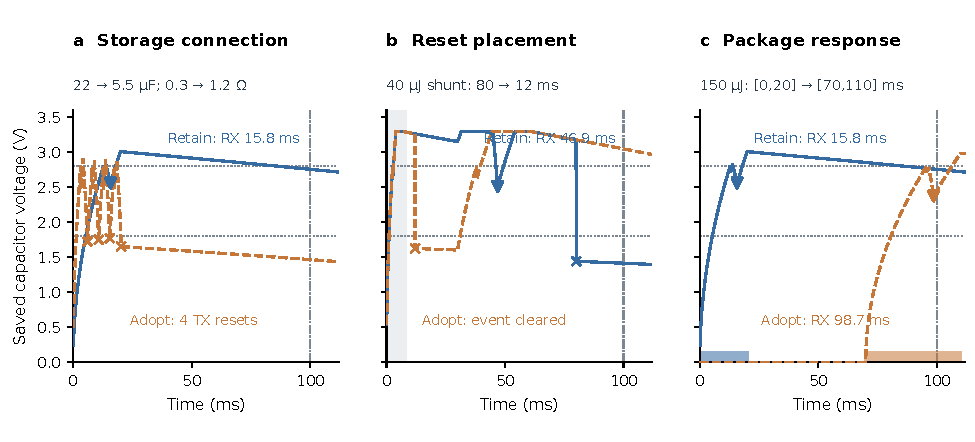
\includegraphics[width=\linewidth]{figures/mechanism-traces.pdf}
\caption{Frozen mechanism changes and saved post-step capacitor voltage.
Blue solid is retain; orange dashed is adopt. Triangles mark actual first
reception and crosses mark saved brownouts; dotted horizontal lines are the
2.8/1.8 V ready/off thresholds. The vertical dash-dot line is the 100 ms
deadline. (a) Series-equivalent storage produces four interrupted transmissions.
(b) Moving the shunt before TX clears volatile pending state; grey shading is
the eight-millisecond contact window. The retain reset is after delivery.
(c) Coloured strips mark prescribed source windows; the delayed intervention
still receives at 98.7 ms. These are five distinct digital exact inputs, with
the common retain trace reused in (a) and (c), not six physical experiments.}
\label{fig:abc-mechanisms}
\end{figure}

\subsection{Storage connection changes the buffer available to one transmission}
The storage family changes two identical ideal cells from parallel to series
while holding the PMIC clamp at 3.3 V. With per-cell capacitance $C_c=11~\mu$F
and ESR $R_c=0.6~\Omega$, the static equivalents are
\begin{equation}
 (C_{\parallel},R_{\parallel})=(2C_c,R_c/2),\qquad
 (C_{\rm series},R_{\rm series})=(C_c/2,2R_c).
\end{equation}
Thus capacitance changes from 22 to $5.5~\mu$F and ESR from 0.3 to
$1.2~\Omega$. The prescribed 7.5 mW source lasts 20 ms in both inputs;
the ideal passive event latch is unchanged. This mapping does not model cell
balancing, voltage-rating changes, leakage mismatch or package parasitics.

Retain receives at 15.8 ms. Adopt boots earlier, begins transmitting at 4.3 ms,
and resets at 6.1 ms before completing the two-millisecond frame. Four
transient resets occur by 20.2 ms and no valid frame arrives. Independent
energy conservation passes, while event reception and transient-voltage service
fail. Earlier readiness and adequate source integral are therefore insufficient
for this transaction. The stored energy above the off threshold, boot work,
ongoing harvest and loaded-rail guard jointly govern completion. A proxy that
compares only capacitor energy with TX work is not an exact failure theorem
when the source can replenish energy during TX.

\subsection{Reset placement changes event availability without changing its energy}
The reset family retains $10~\mu$F storage, a volatile event selector, a contact
from 0 to 8 ms, and earliest TX at 45 ms. Two source pulses supply
210~$\mu$J in total. The intervention moves the same 40~$\mu$J shunt
from 80 to 12 ms; it does not change its integral or insert another event.
Both trajectories first boot at 2.7 ms and capture the event during the contact.

Retain completes delivery at 46.9 ms, before its 80.1 ms reset. Adopt resets
at 12.1 ms, after contact has ended and before transmission is permitted.
Its volatile pending state is cleared. A second boot at 38.1 ms cannot recapture
an already ended contact; no frame is sent. Both independent energy and
receiver-integrity checks pass, but the intervention's event-reception
predicate fails. The discriminating object is the ordering of capture,
state-clearing reset and send, together with the actual reset semantics.
A post-delivery reset in retain does not demonstrate that volatile memory
preserves an undelivered event across reset.

\subsection{Package response changes usable time while preserving total input}
The package family transforms the prescribed rectangular source from
7.5 mW on $[0,20]$ ms to 3.75 mW on $[70,110]$ ms. Both provide
150~$\mu$J. Device parameters, event at zero, passive mechanical latch
and deadline are unchanged. The late input first boots at 95.8 ms and receives
at 98.7 ms, leaving 1.3 ms before the deadline; both retain and adopt pass.

This case is deliberately reported as a passing intervention. The shift does
not imply failure merely because it resembles a late pulse. Conversely, total
energy alone does not establish its tight reception margin. The passive latch
allows the event to remain available before electrical startup. The input
transformation is an assumed package-response law applied to the existing
port model; it is not a measured mechanical transfer function or a new
load-dependent source model. All family judgments remain digital and
physically uncalibrated~\cite{abcb}.
\FloatBarrier

\section{From a missing relation to an executed consumer}
\subsection{A bounded observation language and external qualification}
The observation interface makes the information path explicit
(Figure~\ref{fig:chain}). The participant can list and acquire permitted
sources, propose either a selected field or a constructed relation, and
submit a typed design policy. A proposal states the source identifier,
JSON Pointer paths, units, applicability domain and intended relation.
Selecting a supplied field and constructing a new expression are recorded
as different operations. Neither label alone establishes a new physical
fact or a novel scientific relation~\cite{contract,adapter}.

\begin{figure}[htbp]
\centering
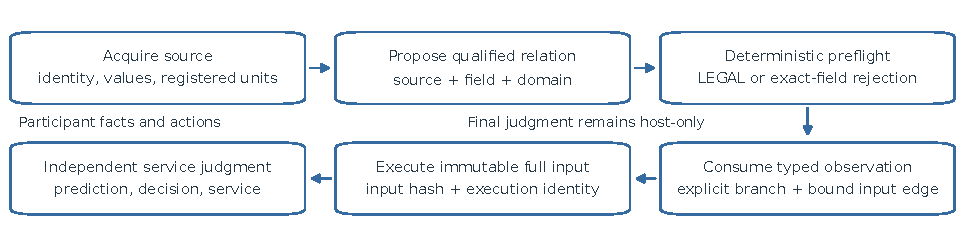
\includegraphics[width=\linewidth]{figures/consumer-chain.pdf}
\caption{The observation-to-consumer chain. Rejection can stop the chain
before any final service execution. Every attempted action and its cost remain
recorded. A source-bound value or a consumed observation alone is not service
or benefit evidence.}
\label{fig:chain}
\end{figure}

Construction uses a bounded JSON abstract syntax tree rather than arbitrary
Python. The interpreter admits at most 64 nodes, depth eight, an 8 MB JSON
source and 32,768 vector elements. A construction must contain a source
field and an allowed operator. Unit dimensions must agree across operations;
the declared output unit must match the root, and declared numeric domain
constraints are checked against source values. Missing fields, unsupported
domains and invalid arithmetic lead to rejection or UNKNOWN. These limits
bound interpretation; they do not calibrate the supplied source.

Authority is outside the proposer. The host binds the original source bytes,
proposal code and input, provider/run identity and actual accounting. An
independent interpreter checks the source relation. A proposer cannot
qualify its own output by supplying an authority record or a success label.
The consumer receives only an admitted observation and the original policy,
then chooses among at most three strictly typed equality branches. Boolean
true and a numeric duration are different values. The complete selected
input, observation edge and actual execution identity are preserved before
the separate service verdict is read~\cite{contract,posthoc,adapter}.

This design distinguishes acquisition from consumption. Echoing a value in
a report is insufficient. A valid consumption receipt shows how that value
entered the executed design. It still does not establish causal necessity:
the same design might be chosen with complete static inputs, and an
observation can be consumed without changing the design. A claimed benefit
would require a separately frozen comparison of alternatives with the same
task and allowance.

\subsection{A concrete constructed relation and its actual consequence}
An earlier actual E5 attempt acquired component, excitation and saved-activity
records, then constructed an energy comparison. Its first proposal omitted
the leading slash required by JSON Pointer. The original host counted that
invalid proposal against the one-proposal limit; the model's already generated
correction was then rejected at the cap. The live attempt remains rejected:
no qualified observation, no real consumer execution, and no proposed-design
scientific execution. Its six SETTLED requests and USD~0.0644115 upper-bound
rate estimate remain charged~\cite{original}.

A separately authorized record labeled
\path{POSTHOC_HOST_ADAPTER_REEVALUATION} later evaluates that existing
corrected call. It makes no new model request and does not replace the
failed live attempt. The model's retained relation is
\begin{align}
 E_{\rm TX}&=I_{\rm TX}\Delta t_{\rm TX}V_{\rm out}=28.8~\mu\mathrm J,\\
 E_{\rm reserve}&=\tfrac12 C(V_{\rm ready}^2-V_{\rm off}^2)=23.0~\mu\mathrm J,\\
 b&=[E_{\rm TX}>E_{\rm reserve}]=\mathrm{true}.
\end{align}
The supplied record uses 8 mA, 2 ms, 1.8 V output, $10~\mu$F capacitance
and 2.8/1.8 V ready/off thresholds. The source-bound domain allows
$4$--$22~\mu$F and $0$--$45$ ms earliest TX, with TX current fixed at
the record's value. A separate Decimal interpreter agrees on the Boolean
and verifies source dependence over legal capacitance values. The
qualification criterion was revised post hoc from a paired-world-specific
test to dependence across legal design values. That intervention and its
scope remain explicit~\cite{posthoc}.

Before an admitted observation, the consumer keeps UNKNOWN and the original
$10~\mu$F, 45 ms design. Qualified Boolean true selects the model's
original $15~\mu$F, 45 ms branch. The actual full service changes from
FAIL with no received frame to PASS with first reception at 46.9 ms. Both
energy ledgers pass, so the energy flag alone cannot explain service. The
selected design avoids a pre-deadline brownout; it does not demonstrate
retention of a pending event across one. A complete static-information
design already passes at $10~\mu$F and 0 ms, receiving at 5.6 ms.
The unused false branch's service is not established by these
receipts~\cite{posthoc}.

The relation is therefore a concrete derived fact that reaches a real
design consumer and has an executed engineering consequence. It is not
prospective live-E5 success, a physical measurement, proof that capacitance
must increase, or an advantage over complete static information. Its
energy inequality omits startup work, losses and event order and cannot
serve as a complete service evaluator. Later adapter-v2 regression records
reject malformed syntax before charging the valid-proposal counter, while
bounding syntax rejections and retaining a one-valid-proposal limit. Those
new-version checks preserve the original failure~\cite{adapter}.
\FloatBarrier

\section{Legal input before real consumption}
\label{sec:abc-contract}
\subsection{Source identity, units and conditions are separate from a verdict}
The additive \path{abc-e5-input-v1} protocol addresses the two admission
failure classes exposed by the old E5 records. Each source leaf states its
source identifier and JSON Pointer. The host binds source bytes, a fixed unit
registry and the immutable current/intervention context. Each domain row
names its own source, so a component capacitance and an excitation deadline
need not incorrectly share a single source-local unit map. A source from
another candidate context or an inapplicable source condition is rejected
before execution~\cite{gateways,abcfirst,abcaudit}.

Values are interpreted in the registered source units, then converted to
compatible output and consumer units. For example, a farad-valued source can
be bounded using microfarads without reinterpreting its stored number as a
microfarad value. Numeric bounds and equality conditions are normalized before
comparison. Incompatible dimensions, unavailable fields and invalid conditions
produce a structured rejection naming the failing request field. The bounded
expression interpreter and separate Decimal source-algebra check are reused;
they do not read hidden service truth.

Boolean, numeric and string types remain distinct. A Boolean relation cannot
implicitly select numeric-duration branches. If a designer intends that
mapping, it must explicitly provide the true/false numeric values and units;
prefix conversion then occurs before strictly typed branch matching. For
example, an explicit true-to-2-ms mapping can match a 0.002 s branch. Omitting
the mapping is an input-type error. The protocol repairs representational
friction without silently changing a proposed consumer's meaning.

A LEGAL response means that the specified source relation, domain and consumer
are consistent on that frozen input. It does not establish that the relation
is necessary or sufficient for complete service over the whole declared range.
Numerical agreement between two interpreters is not an independent proof of a
scientific hypothesis. Final independent energy and receiver checks therefore
remain outside preflight and outside the participant's final evaluator access.

\subsection{The actual observation edge and the independent service edge}
A legal relation reaches the consumer through a stored typed value and branch.
The host records source bindings, normalized relation, selected decision,
observation-to-input edge, full executed-input hash and execution identity.
Only the selected immutable retain/adopt task can be dispatched. An input
binding mismatch stops execution; a reported scalar without that edge is not
counted as actual typed consumption. The same real executor and independent
receiver/energy checks serve all arms. Fixture software tests are explicitly
excluded from scientific evidence~\cite{abcaudit}.

The separate development rehearsal demonstrates that this path is usable.
A researcher supplies the earlier TX-versus-reserve relation, now bound to
component and excitation sources with explicit conditions. Boolean true reaches
the actual consumer and selects the frozen $15~\mu$F intervention; reception
occurs at 46.9 ms and selected service passes, while the current design fails.
No model request is made. The submitted prediction is intentionally UNKNOWN,
so prediction coverage is false even though typed consumption and selected
service are established. The rehearsal is excluded from all eighteen formal
attempts and establishes neither autonomous discovery nor comparative
advantage~\cite{abcfirst}.

Formal participants can also directly submit a decision. This route is legal
for every arm, including refinement. A valid direct prediction and selected
passing input are scientific outcomes even when no typed relation is consumed.
Consequently the conjunction called \path{interface_decision_success} in the
host record is a path-specific diagnostic. It is not the main success metric
and cannot be used to penalize a complete-information baseline for choosing
a correct design directly. Source legality, path use, scientific judgment,
service and budget completion are reported independently in the new results.
\FloatBarrier

\section{Earlier matched digital experiment}
\subsection{Tasks, outcome and strong controls}
The main comparison uses four fixed tasks. Pulse-fast is a static-sufficient
control. Volatile-reset and latched-reset use the transient BF apparatus
with different pending-state semantics. Their legal design variables are
capacitance and earliest permitted transmission, under frozen task-specific
ranges. Complete service uses independent energy and receiver checks plus
the registered ordered-event analysis. PASS denotes admitted complete
service, FAIL an admitted final design that fails it, and INCOMPLETE no
admitted final execution~\cite{protocol,comparison}.

The fourth task is a preregistered C-lite single-query derivative. It supplies
20~$\mu$W ideal DC for 30 s, 1~$\mu$W idle load, zero initial energy and
a 50~$\mu$J reply. A query at 2 s must receive its matching reply by 7 s
with maximum data age 5 s. Capacitance is $25$--$100~\mu$F at an ideal
2 V ceiling; ESR, boot energy and boot delay are zero and harvest efficiency
is one. Gates require query issuance, capture, matching token, causal order,
deadline and freshness. The fixed token value 1 represents one virtual
query, not a secure multi-query protocol or an RF environment. These are
explicit synthetic assumptions~\cite{derivative}.

Average-energy begins with the coarse source integral and average power.
Rich-static and complete-input supply all input records and the full
model definition. They have the same available facts in this registered
comparison, making their tie an admissible control. The saved condition
name for complete-input is \path{complete-raw}; it does not mean that the
participant receives the full coupled physical trace. That trace is
host-side audit material. Executable-response adds candidate-specific
public energy ledgers, activity and packets. Live E5 begins coarse and
actually acquires permitted records, proposes a field or relation, obtains
external qualification and submits a typed consumer policy. No target
expression, required-field list or answer-bearing relevance label is
prefilled~\cite{protocol,tables}.

E4 changes only the rich-static initial serialization, comparing JSON with
a typed JSON-Pointer table. The table preserves nested containers, types
and empty values. All twelve formal pairs have saved receipts of identical
decoded initial packets and tools. Later source responses use common JSON
in both arms. This is an initial-serialization comparison rather than a
representation intervention across the whole interactive trajectory.

\subsection{Repetitions, resource parity and cache exposure}
Two pilot repetitions on volatile-reset precede the formal comparison.
The registered one-time instability rule selects three formal repetitions,
then freezes that count. Pilots remain separate development evidence.
The full eight-condition matrix contains 112 unique groups and 140 actual
episodes: 96 formal groups and 16 pilot groups. Parent method proposals
account for additional episodes in two conditions. This paper displays
six interface conditions, covering 72 formal and 12 pilot groups. Rich-static
is also E4 JSON, and complete-input is also the fixed-method cell; these
shared cells are counted once~\cite{protocol,comparison}.

Within each compared task, the scientific laws, service evaluator, legal
design domain, reported model alias, initial cache and total resource caps
remain fixed. Information access varies as declared by the condition.
Each group has 24 provider requests, 40 tool calls, 1,200 s and at most
two distinct design exposures, counting checks, response queries and
confirmation. Acquisition, qualification and consumption do not add a
free E5 budget. A parent proposal, when present, has an eight-request,
400 s sublimit within the group. The campaign caps are 3,000 requests,
USD~200 in settled conservative estimates and 134,400 summed episode
seconds. Failed groups are not automatically retried or replaced.

Every group starts from one immutable cache containing twelve exact-input
responses and one registered derivative baseline. Private overlays isolate
new job histories. A cache hit still consumes logical design exposure;
it does not reveal another group's output before a query or enlarge the
two-design cap. The records' term ``physical cache'' denotes the underlying
digital execution cache and supplies no laboratory evidence. Fresh
participant entries and the common cache identity are retained per group.
The model is reported as \path{deepseek-flash}; this alias does not establish
a pinned weight identity~\cite{comparison}.

\subsection{Preparation and negative controls}
The structural preparation separately exports 64 inputs across four cases,
four information levels, two formats and two observation regimes. Thirty-two
format pairs preserve decoded facts, assets, tools and resource limits.
These are preparation checks, distinct from actual model trials. Fixed
parser checks abstain on all four current-only cases and correctly judge
all four sufficient-information cases in both supplied serializations.
They do not measure language-model comprehension~\cite{structural,contract}.

Negative controls retain the enriched static solution, complete raw model,
uninformative observation, exhausted acquisition budget, illegal design
changes and tampered source binding. A researcher-specified required-field
selector and a researcher-supplied headroom expression are construction
baselines, not autonomous discoveries. Preparation outcomes are not
substituted for later live completion, and software validation of a
consumer edge is not promoted to hardware acceptance.

\section{New equal-access intervention comparison}
\label{sec:abc-protocol}
\subsection{Frozen tasks and strong baseline information}
The new finite list comprises the three tasks in
Section~\ref{sec:abc-mechanisms}, three assigned arms and two fresh-context
repeats per task: eighteen formal attempts, six per arm. It is not a new
eighteen-task benchmark. The mechanism families, exact retain/adopt inputs,
arm instructions and repeat identities are frozen before new task execution;
sampling phase is reserved and excluded. Neither the researcher-provided
development request nor another arm's answer is placed in formal context.
No task is replaced after its outcome~\cite{abcb,abcaudit}.

Complete information receives the full source payload initially and can use
all tools. The fixed-rule control checks ready/off and loaded-rail feasibility,
usable energy during the operation, event availability across any reset, and
deadline. It is a conservative classical rule set, not a deliberately weak
average-energy control. Refinement is instructed to identify an activated
mechanism, acquire the corresponding sources and conditions, and express a
relation that drives the typed consumer. It can also submit directly. The
assigned arm is retained regardless of the actual path taken.

All arms have the same complete source catalogue and execution permissions:
component records, excitation records, full current/intervention inputs and
the unchanged numerical model law. Every arm can acquire the entire catalogue
in one call and can use preflight, checks or direct submission. Initial context
serialization and the method instruction differ by design; identical source
availability is not a claim of byte-identical initial prompts. The audit checks
source payload parity and within-task scientific inputs. Initial payload volume
and subsequent acquisition are therefore accounted separately.

\subsection{Common resources, hidden checks and outcome definitions}
The common ceilings are twelve model requests, forty tool calls, 900 s and two
distinct immutable designs. Source acquisition, invalid attempts, preflight and
rework all consume the same episode allowance. Maximum output is fixed at
65,536 tokens for this new batch after backend qualification; it does not
rescue or remove the four older 32,768-token censored O episodes. All formal
participants use fresh contexts and the reported alias \path{deepseek-flash}.
The underlying weight identity remains UNKNOWN~\cite{abcaudit}.

The participant predicts PASS, FAIL or UNKNOWN for the intervention and chooses
adopt or retain. The registered decision rule is adopt if the intervention
passes, otherwise retain; retain is therefore not automatically the correct
answer for the passing package task. Independent host evaluation checks both
fixed inputs after the public endpoint closes, filling an unexecuted input
through the same exact-input executor. No hidden final verdict is a tool action.

We retain five distinct measurements: actual artifact submission; prediction
coverage and correctness; decision correctness and selected service; actual
typed consumption; and original normal-completion status. A request-cap stop
can follow an actual submission, so an incomplete runtime status does not imply
that no artifact exists. Budget-compliant service requires both the original
normal-completion status and an independent service pass. Every assigned row,
including stopped rows, remains in the six-per-arm denominator.

\subsection{Execution and cost accounting}
The exact-input cache preserves one canonical raw artifact per input. Each
episode's host evaluation exposes two inputs, regardless of whether one or
both are cache hits. We report evaluated-input references, cache reuses and new
scientific calculations separately. Later arms inherit a warmer shared cache;
zero new calculation in those arms is a schedule effect, not an algorithmic
advantage. A cache hit supplies no free extra candidate or automatic retry.

Cost views retain requests, input/output/reasoning tokens, initial payload
volume, acquired bytes, preflight/reject counts, tool time and total wall time.
Host evaluation is included in total episode wall time but lacks a separately
recorded duration. We do not infer an exact host-only time by subtraction.
The reported fee is a conservative fixed-rate estimate on settled usage,
not an invoice. Codex preparation cost remains UNKNOWN. With only three fixed
tasks and two contexts per task, comparisons are descriptive; no significance,
population equivalence or generalization claim is made.
\FloatBarrier

\section{Earlier results: the strong static control}
\subsection{The complete-service comparison}
Table~\ref{tab:formal} reports every formal group. Average-energy yields
8 PASS and 4 FAIL. Rich-static, complete-input, executable-response and
E4 table each yield 12 PASS. Live E5 yields 7 PASS and 5 INCOMPLETE;
it has no admitted final service FAIL. Its completion rate is 7/12,
not a conditional 7/7. Missing final executions and submitted service
failures remain different outcomes with the same full denominator.

% Generated from hash-verified saved data; no scientific execution.
\begin{table}[htbp]
\centering\small
\caption{Formal matched interface comparison: four fixed tasks, three repetitions per task, twelve groups per arm. P/F/I are PASS, submitted FAIL and INCOMPLETE. Every incomplete group and its requests remain included.}
\label{tab:formal}
\begin{tabular}{@{}lrrrrr@{}}\toprule
Condition & P & F & I & Requests & Requests/group \\\midrule
Average energy & 8 & 4 & 0 & 75 & 6.2500 \\
Rich static / E4 JSON & 12 & 0 & 0 & 65 & 5.4167 \\
Complete input & 12 & 0 & 0 & 64 & 5.3333 \\
Executable response & 12 & 0 & 0 & 66 & 5.5000 \\
Live observation (E5) & 7 & 0 & 5 & 80 & 6.6667 \\
E4 typed table & 12 & 0 & 0 & 65 & 5.4167 \\
\bottomrule\end{tabular}
\end{table}

% Generated from hash-verified saved data; no scientific execution.
\begin{table}[htbp]
\centering\small
\caption{Formal P/F/I out of three per task. Each strong arm separately denotes rich static, complete input, executable response and E4 table; none has an omitted failure.}
\label{tab:tasks}
\begin{tabular}{@{}lccc@{}}\toprule
Fixed task & Average energy & Live E5 & Each strong arm \\\midrule
Pulse-fast & 3/0/0 & 2/0/1 & 3/0/0 \\
Volatile reset & 1/2/0 & 2/0/1 & 3/0/0 \\
Latched reset & 1/2/0 & 1/0/2 & 3/0/0 \\
C-lite query derivative & 3/0/0 & 2/0/1 & 3/0/0 \\
\bottomrule\end{tabular}
\end{table}


The coarse arm's observed deficit occurs in the two reset tasks, each
with one PASS and two FAIL. Pulse-fast and the C-lite derivative each
have three PASS. Every strong arm passes all three repetitions on each
task (Table~\ref{tab:tasks}). This finite result is consistent with the
value of supplied timing and state information beyond the coarse energy
summary. It establishes no service advantage for executable-response
over rich-static information. The saturated controls also do not prove
equivalence on harder or previously unused tasks.

The two pilot repetitions are not pooled with the formal twelve. On
their single volatile-reset input, average-energy has one PASS and one
FAIL; each other displayed arm has two PASS. E5's two pilot completions
include one selection and one construction. These are the development
observations preceding the one-time formal-repeat freeze, not additional
formal successes or independent tasks~\cite{tables,protocol}.

\subsection{What the seven prospective E5 chains did}
Every formal E5 completion contains an actual prospective proposal,
external source qualification and a typed observation consumed by the
design policy. Six select existing fields and one constructs a relation.
Five use component records and two excitation records. Six change the
initial design and one does not. All seven final designs pass independent
service, and all seven deliver before any reset. Their successes therefore
establish neither pending-state survival across a reset nor the necessity
of the acquired observation. New physical measurements number
zero~\cite{tables,comparison}.

% Generated from hash-verified saved data; no scientific execution.
\begin{table}[htbp]
\centering\small
\caption{Disposition of all twelve formal E5 groups. Repeated rejected actions are not additional groups; absent executions are retained as INCOMPLETE.}
\label{tab:e5}
\begin{tabular}{@{}lrc@{}}\toprule
Disposition & Groups & Final service \\\midrule
Qualified selection, consumed & 6 & PASS \\
Qualified construction, consumed & 1 & PASS \\
Source-unit binding rejected & 4 & INCOMPLETE \\
No typed consumer match & 1 & INCOMPLETE \\
\bottomrule\end{tabular}
\end{table}


Four incomplete groups retain \path{SOURCE_UNIT_UNAVAILABLE} in their
original gateway records. The code identifies a submitted source/field/domain
unit-binding problem; it does not imply that a physical quantity does not
exist. In the pulse-fast example, the selected packet field
\path{/packets/0/application_bytes} is unit-mapped in the acquired
saved-activity source, while the declared domain also references deadline,
TX-duration and readiness fields absent from that source's unit map.
A latched-reset proposal selects a packet field from the model-law source,
whose mapped fields describe model identity and Python definition.
The original generic error does not name the first rejected term.
We diagnose the source-local mismatch from saved proposals and logs;
no repaired proposal is evaluated~\cite{gateways}.

The fifth incomplete group records \path{NO_TYPED_CONSUMER_MATCH} on
the C-lite derivative. Its equality expression outputs a Boolean while
the consumer branches match numeric durations 0.002 and 0.001. A value
can therefore be syntactically meaningful yet fail to enter the intended
design edge. Other syntax and valid-proposal-cap errors remain charged
actions inside these groups, not extra independent trials or free
rescue attempts. Table~\ref{tab:e5} counts groups once.

The rejected original E5 attempt and its separately authorized post-hoc
adapter chain remain outside these twelve formal groups. The post-hoc
record demonstrates engineering linkage of an already generated relation.
The seven later formal completions demonstrate prospective operation
under a different registered protocol. Relabeling the former as a
successful live discovery would erase both its original admission
failure and the host intervention~\cite{original,posthoc}.

\subsection{Equal information and acquisition overhead}
E4 gives identical complete-service and request totals: JSON and the
typed table each pass 12/12 using 65 provider requests, or 5.4167 per
group. The retained USD and wall receipts differ
(Table~\ref{tab:format}), but this small comparison isolates neither
all latency determinants nor the representation of later acquisitions.
It supplies no observed service or request advantage and no causal
format-speed or format-cost conclusion~\cite{tables}.

% Generated from hash-verified saved data; no scientific execution.
\begin{table}[htbp]
\centering\small
\caption{E4 equal-information initial serialization. Later acquisitions use common JSON. Cost and summed group wall time are descriptive; neither establishes a format advantage.}
\label{tab:format}
\begin{tabular}{@{}lrrrr@{}}\toprule
Initial packet & PASS & Requests & USD & Wall (s) \\\midrule
JSON & 12/12 & 65 & 0.4267200 & 676.5 \\
Typed table & 12/12 & 65 & 0.5145681 & 611.4 \\
\bottomrule\end{tabular}
\end{table}

% Generated from hash-verified saved data; no scientific execution.
\begin{table}[htbp]
\centering\small
\caption{Finite observation selection on four exposed cases. Read and audit bytes are Python payloads, not disk I/O. Host timings are single historical measurements, not latency benchmarks; selected and mechanism-spec contain the same facts.}
\label{tab:acquisition}
\begin{tabular}{@{}lrrrrr@{}}\toprule
Observation & Correct & Read B & Audit B & Wall ms & Model runs \\\midrule
uninformative & 0/4 & 4648 & 4648 & 0.289 & 0 \\
mechanism-spec & 4/4 & 103 & 103 & 0.260 & 0 \\
fixed-rich & 4/4 & 4747 & 4747 & 0.282 & 0 \\
full-raw & 4/4 & 8544 & 8544 & 0.333 & 0 \\
executable-dynamic & 4/4 & 8544 & 8544 & 1.886 & 4 \\
selected & 4/4 & 103 & 103 & 0.236 & 0 \\
\bottomrule\end{tabular}
\end{table}


The earlier finite observation selector chooses the smallest eligible
source using researcher-supplied required-field metadata, without service
outcomes. It reads the same 103 bytes and facts as the fixed mechanism-spec
baseline; both correctly judge four cases. Rich-static, complete raw and
an executable response also correctly judge all four. The historical
timings in Table~\ref{tab:acquisition} include acquisition and source
audit, plus selection when used. They are single-host payload measurements
with uncontrolled cache state, not storage-I/O or monetary measurements.
Thus lower payload volume relative to a full model is not an independent
selection-algorithm gain~\cite{structural}.

A deterministic compiler also constructs the researcher-specified
headroom observation. Its saved outputs of $-14$ and $8~\mu$J agree
with twenty exposed clamp-grid checks and two fresh-process executions.
Construction took 0.239 ms, reference qualification 13.017 ms and the
two fresh processes 37.730 ms combined in those retained receipts.
Because the equation and relevant fields were supplied by a researcher,
this is executable construction machinery, not an autonomous discovery.

\subsection{Service success versus an ordered retention witness}
Four formal participant groups select a pending-event-across-reset result:
two complete-input groups, one proposed-method group and one E4 table
group. They make four fresh choices but reuse one distinct historical
digital execution key. All select $10~\mu$F and earliest TX at 45 ms.
The same event is captured from 3.7 to 7.9 ms, a brownout occurs at
12.1 ms, and first valid reception follows at 46.9 ms. The fixed ideal
passive latch provides the retention mechanism~\cite{ordered}.

All twelve rich-static, all twelve executable-response and all seven
successful E5 groups instead deliver before any reset. Their complete
service passes are valid for their tasks but are not evidence for the
stronger ordered-retention property. Conversely, four selections of one
response are not four independent physical experiments or four newly
invented retention mechanisms. The ordered audit creates zero new
scientific executions and retains physical qualification UNKNOWN.
\FloatBarrier

\section{New results: legal consumption without an outcome advantage}
\label{sec:abc-results}
\subsection{All three assigned arms reach the correct scientific decision}
Table~\ref{tab:abc-outcomes} uses all eighteen frozen attempts. Each arm
has six actual decision artifacts, six correct predictions, six correct
adopt/retain decisions and six independent selected-service passes. All
intervention predictions have coverage. There are no wrong adoptions or
rejections. Every context rejects the storage and reset interventions and
adopts the passing package intervention. The complete-information baseline
therefore leaves no observed scientific-accuracy deficit for refinement to
remove on this finite task list~\cite{abcb,abcreview}.

\begin{table}[tbp]
\centering\small
\setlength{\tabcolsep}{4.5pt}
\caption{New formal outcomes, each out of six assigned attempts (three tasks, two fresh contexts each). Actual submission is distinct from normal budget completion. Pred., Dec. and Svc. denote correct intervention prediction, correct adopt/retain decision and selected-service PASS. Typed is only a path statistic.}
\label{tab:abc-outcomes}
\begin{tabular}{lrrrrrr}
\toprule
Assigned arm & Actual sub. & Pred. & Dec. & Svc. & Budget & Typed \\
\midrule
Complete information & 6/6 & 6/6 & 6/6 & 6/6 & 6/6 & 1/6 \\
Fixed conservative rules & 6/6 & 6/6 & 6/6 & 6/6 & 4/6 & 4/6 \\
Observation refinement & 6/6 & 6/6 & 6/6 & 6/6 & 6/6 & 3/6 \\
\bottomrule
\end{tabular}
\end{table}


Normal budget completion is a separate outcome. Complete information and
refinement each finish normally in six attempts; fixed rules finish normally
in four. The first fixed-rule repeats on reset placement and package response
each reach twelve settled requests and retain
\path{INCOMPLETE_OR_STOPPED}. Before stopping, both have an actual direct
submission with a correct prediction and decision and selected-service PASS.
They are neither missing submissions nor normally completed episodes. Their
full costs and the original stop labels remain in the table denominator.

Actual typed consumption occurs in one complete-information attempt, four
fixed-rule attempts and three refinement attempts. The other decisions are
legal direct submissions. In particular, three refinement attempts do not
complete the proposed typed path but do reach the correct engineering
decision. They remain in the assigned refinement arm; no replacement episode
is run. The 1/4/3 counts describe use of an optional path, not relative
scientific success. Applying the path-specific conjunction to all arms would
incorrectly penalize a strong direct baseline.

\subsection{What a formal typed observation establishes}
The refinement reset example binds event/contact and transmission timing from
complete inputs to the shunt time in the excitation source. Its Boolean result
is false and is actually read by the retain branch. The stored edge identifies
both source hashes, the typed value and the executed current-input hash.
The independent saved trajectories then establish why retain passes and adopt
fails: the 12.1 ms intervention reset clears the volatile event after the
contact ends, whereas the current input sends before its late reset.

The passing package example also consumes a Boolean, now true, and selects
adopt. Its proposed relation combines pulse start, deadline, boot delay, TX
duration, power and efficiency with the energy needed to reach the ready
threshold. The independent executor supplies the actual 98.7 ms reception.
The source calculation is a qualified intermediate fact; the final service
check additionally covers event availability, loads and reception. Correct
service on this one input does not prove that the proxy is sufficient over
every numeric bound in its declared domain.

The storage example consumes false and retains parallel storage. Its
energy-window proxy correctly accompanies that decision on the frozen input,
but does not replace the full transient model. In particular, harvest during
TX, boot-step overshoot and the ESR guard must be considered before promoting
such a proxy to an exact criterion. The raw proposal and its explanatory
text are retained as participant outputs; interpreter agreement and a correct
selected outcome do not validate every explanatory statement. No formal
attempt supplies a new physical measurement or establishes universal
autonomous discovery~\cite{abcb,abcaudit}.

\subsection{More requests, equal acquisition and a mixed cost result}
Table~\ref{tab:abc-costs} shows 37, 59 and 50 requests for complete information,
fixed rules and refinement. Each acquires exactly 89,218 logical source bytes
over six attempts. Refinement therefore has no observed acquisition-volume
gain and uses thirteen more requests than complete information. Preflight
calls number 15/34/20 and rejected actions 9/27/14. Improving the admission
schema does not remove operational errors or make extra interaction free.

\begin{table}[tbp]
\centering\small
\setlength{\tabcolsep}{4.5pt}
\caption{New formal resource totals over six attempts per arm. Tokens are total input/output usage; reasoning tokens are not added a second time. USD is the conservative fixed-rate estimate, not an invoice. Acquired bytes are logical source-response bytes, not disk I/O or total context volume.}
\label{tab:abc-costs}
\begin{tabular}{lrrrrr}
\toprule
Assigned arm & Requests & Input tokens & Output tokens & Est. USD & Acquired B \\
\midrule
Complete information & 37 & 1,207,152 & 198,172 & 0.5999520 & 89,218 \\
Fixed conservative rules & 59 & 1,816,101 & 226,434 & 0.8165511 & 89,218 \\
Observation refinement & 50 & 1,157,649 & 176,741 & 0.5593839 & 89,218 \\
\bottomrule
\end{tabular}
\end{table}


The corresponding conservative fee estimates are USD~0.5999520, 0.8165511
and 0.5593839. The calculation uses input and output usage at fixed rates:
\begin{equation}
 \widehat C_{\rm USD}
 =0.30\frac{N_{\rm input}}{10^6}
  +1.20\frac{N_{\rm output}}{10^6}.
\end{equation}
Reasoning tokens are an output-accounting field, not an additional additive
budget. Refinement uses fewer total input and output tokens than complete
information in these receipts despite its larger request count. That yields
the slightly lower fee estimate; it does not make every cost dimension better.
Rates, response length and initial payload volume all enter this descriptive
comparison. The estimates are not invoices and exclude unmetered preparation.

\begin{figure}[tbp]
\centering
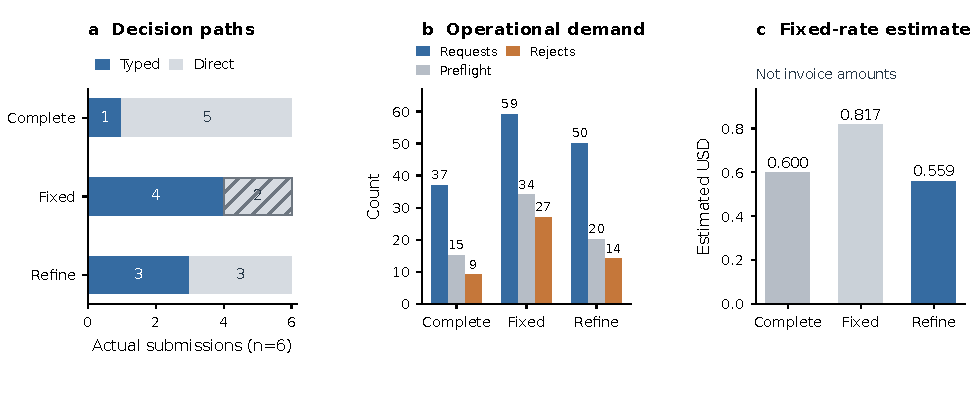
\includegraphics[width=\linewidth]{figures/cost-paths.pdf}
\caption{New formal path and cost comparison, all six assigned attempts per
arm. (a) Typed and direct submissions both count as actual artifacts; hatching
marks the two fixed-rule budget stops after direct submission. (b) Requests,
preflights and rejects are distinct operational counts. (c) Conservative
fixed-rate fees, rounded here to three decimals. All arms independently have
six correct predictions, six correct decisions and six selected-service passes.
Bars are finite totals across three fixed tasks and two fresh contexts per
task; no error bars, significance or population estimate is implied.}
\label{fig:abc-costs}
\end{figure}

\begin{table}[tbp]
\centering\small
\setlength{\tabcolsep}{4.5pt}
\caption{Operational and execution accounting. Initial B is summed initial payload bytes; PF/rej. count preflights/rejected actions. Wall includes host evaluation; no separate host-only duration was recorded. Eval/cache/new count evaluated-input references, cache hits and new scientific computations, respectively. Cache order prevents an algorithmic-savings interpretation.}
\label{tab:abc-accounting}
\begin{tabular}{lrrrrrrrr}
\toprule
Arm & Initial B & PF & Rej. & Tool s & Wall s & Eval & Cache & New \\
\midrule
Complete & 175,414 & 15 & 9 & 0.376 & 870.3 & 12 & 8 & 4 \\
Fixed & 62,054 & 34 & 27 & 0.162 & 926.7 & 12 & 12 & 0 \\
Refine & 61,850 & 20 & 14 & 0.176 & 755.7 & 12 & 12 & 0 \\
\bottomrule
\end{tabular}
\end{table}


All arms have twelve evaluated-input references. Complete information accounts
for four new scientific computations and eight cache reuses; fixed rules and
refinement each reuse twelve cached inputs and add zero computations. Five
distinct exact inputs underlie the three mechanisms because two tasks share
the same current design. The cache is warmer for later arms, so the zero is
not an algorithmic compute saving. Tool time is separately reported from
total wall time, and the unrecorded host-only duration remains unavailable.

The B formal batch totals 146 settled requests, USD~1.9758870 in these
estimates and 2552.7 summed episode seconds. The complete finite cycle has
48 model episodes and 307 settled requests with an estimate of
USD~5.5299957; this already includes B, A and C formation/validation/formal
work and must not be added to their subtotals. The developer rehearsal has
zero model requests and remains outside eighteen~\cite{abcb,abcaudit}.

\begin{table}[tbp]
\centering\small
\setlength{\tabcolsep}{4.5pt}
\caption{Every new formal attempt, with no deletion or replacement. C/F/R denote complete information, fixed rules and refinement. S is normal ACTUAL\_SUBMITTED completion; X is original INCOMPLETE\_OR\_STOPPED. Every row has an actual artifact, correct prediction/decision and selected-service PASS; T indicates actual typed use.}
\label{tab:abc-attempts}
\begin{tabular}{lrrrrrrr}
\toprule
Mechanism & Arm & Repeat & Status & T & Requests & PF & Rejects \\
\midrule
package response & C & 1 & S & 0 & 7 & 3 & 2 \\
package response & C & 2 & S & 0 & 7 & 4 & 3 \\
package response & F & 1 & X & 0 & 12 & 9 & 7 \\
package response & F & 2 & S & 1 & 11 & 6 & 5 \\
package response & R & 1 & S & 1 & 6 & 3 & 2 \\
package response & R & 2 & S & 0 & 10 & 5 & 4 \\
reset placement & C & 1 & S & 0 & 4 & 2 & 1 \\
reset placement & C & 2 & S & 0 & 6 & 2 & 1 \\
reset placement & F & 1 & X & 0 & 12 & 8 & 7 \\
reset placement & F & 2 & S & 1 & 6 & 2 & 1 \\
reset placement & R & 1 & S & 0 & 10 & 4 & 2 \\
reset placement & R & 2 & S & 1 & 8 & 2 & 1 \\
storage connection & C & 1 & S & 1 & 7 & 2 & 1 \\
storage connection & C & 2 & S & 0 & 6 & 2 & 1 \\
storage connection & F & 1 & S & 1 & 10 & 6 & 5 \\
storage connection & F & 2 & S & 1 & 8 & 3 & 2 \\
storage connection & R & 1 & S & 1 & 7 & 3 & 2 \\
storage connection & R & 2 & S & 0 & 9 & 3 & 3 \\
\bottomrule
\end{tabular}
\end{table}


\subsection{Relation to the earlier negative comparison}
The new protocol establishes actual legal consumption under frozen new
mechanisms and preserves all original source/type failures. It does not
retroactively change the earlier seven-pass/five-incomplete E5 result, and
the new six-per-arm scientific outcome cannot be read as a controlled
before/after effect of preflight: task list, resource limits and protocol
version differ. Both studies support the same bounded comparison. Complete
static information is a successful control, and the live refinement route
has not demonstrated additional scientific success. The new study further
shows equal source acquisition, more requests than the strongest control,
and a mixed rather than comprehensive cost advantage.
\FloatBarrier

\section{Event-time service exposes another interface boundary}
\subsection{The original O service and its strong fixed control}
The O study extends the digital apparatus to vibration start, active
keepalive and stop service. O0 is a 21,600 s task with zero initial
capacitor energy, $C=15$ mF and a prescribed source associated with a
$15~\mathrm{cm}^2$ photovoltaic area. Its six intervals have nominal
light levels 200/0/50/200/0/50 lux at boundaries
0/120/150/180/300/330/360 min. The corresponding electrical inputs
are separately prescribed as 90/0/20/90/0/20~$\mu$W; the 3500 K label
is metadata and lux is not converted into watts. RMS vibration is
0.08 g in the four declared activity intervals and 0.005 g otherwise.
These inputs are uncalibrated digital assumptions~\cite{otask}.

Start requires RMS continuously above 0.05 g for 3 s; stop requires
RMS continuously below 0.01 g for 60 s. Equality resets confirmation.
The confirmation instant is the event time. Each start and stop must
arrive within 10 s and carry an encoded timestamp within 1 s; active
keepalive gaps must not exceed 120 s and idle false events fail.
The first dark interval contains one required active interval, so
darkness cannot simply be excluded from service.

The inherited ideal energy path has 0.8 harvest efficiency, 0.38 V/
3~$\mu$W cold-start gates, 2.7/2.3 V ready/off thresholds, 3.3 V
maximum capacitor voltage, 5.5 V rating and $0.3~\Omega$ ESR.
It supplies 1.8 V with 0.3 V dropout, 1/5~$\mu$W off/sleep power,
100~$\mu$J boot and 130~$\mu$J atomic TX transactions. Added RMS
costs are 0.5~$\mu$W standby, 1~$\mu$J wake, 20~$\mu$J per
successful sample and 5~$\mu$J per committed write. The write is
not charged at every poll. These proposed costs do not qualify a
vibration sensor, PMIC, clock, NVM or RF receiver.

O0 compares a free legal candidate, a fixed 60 s periodic snapshot
control and a fixed rich-state start/stop machine. They share the
same task, source, hardware and event evaluator. The candidate and
rich-state control submit the same one-second, NVM,
\path{confirmed_events} program with the same thresholds, one-second
retry and zero backoff. They share an exact execution key and
response, match eight events, deliver 18 accepted packets and pass
the nominal O predicate. The periodic control delivers 348 accepted
packets and passes energy, but matches no required event. It fails
service~\cite{o0}.

% Generated from hash-verified saved data; no scientific execution.
\begin{table}[htbp]
\centering\small
\caption{Original O0 development task. Candidate and rich-state control share one exact design and response. Self-judgment is scoped separately from the host O event predicate.}
\label{tab:o0}
\begin{tabular}{@{}lrrccr@{}}\toprule
Arm & Poll (s) & Matched/8 & Host O & Self-judgment & Requests \\\midrule
candidate & 1 & 8/8 & PASS & UNKNOWN & 8 \\
fixed-periodic & 60 & 0/8 & FAIL & FAIL & 5 \\
rich-state & 1 & 8/8 & PASS & PASS & 5 \\
\bottomrule\end{tabular}
\end{table}


The candidate checks one-second sampling, then 1.5-second sampling,
and ultimately submits the former. In the retained 1.5-second
alternative, the first start is observed at 4204.070423 s and stamped
4204.139063 s against truth 4203 s. The stamp error 1.139063 s
exceeds tolerance even though energy and delivery can appear
adequate. This checked alternative is preserved in the same episode's
exposure and cost history, not treated as a later repair to its
accepted design~\cite{o0}.

The candidate's own judgment is UNKNOWN. Its original explanation
concerns unobserved dark intervals after brownout, absent gap-report
messages, inherited A/R first-report and dark-report metadata, and
unavailable source/hardware calibration. In particular, inherited
metadata calls for reception by 1800 s and dark reporting every
600 s, while the first confirmed O event is later. The host's O
predicate asks a narrower event-service question and returns PASS.
Its saved disagreement flag is nominal to that predicate. This is
not evidence of a mistaken physical-acceptance judgment. Neither
the flag nor O PASS discharges inherited reporting obligations.
The observed brownouts near 8766.18 and 19587.64 s occur after
required active intervals; success on this waveform does not
establish uninterrupted six-hour sensing~\cite{o0,otask}.

\subsection{A frozen new waveform and complete denominators}
A secondary closed comparison freezes six descendant design procedures
before any final input. Fixed H0 is unchanged; G0 is a fixed
procedure improver; G1 is one actually proposed improver. Three paired
descendant lineages are conditional on that single G1 formation,
not three independent G1 training runs. Thirty effective selection
cells pass before freezing. Each final design episode then sees the
complete current task, including its waveform. ``Unexposed'' describes
formation and selection, not concealment of the waveform from the
final designer~\cite{transfer}.

Each arm has nine final cells: three lineage contexts on each of
two reserved digital tasks and a new O waveform. Both digital tasks
pass in all eighteen cells. The complete 27-cell totals are H0
7/1/1, G0 6/1/2 and G1 8/0/1 in PASS/submitted-FAIL/INCOMPLETE
order. The O rows account for all differences
(Tables~\ref{tab:finalarms} and~\ref{tab:ofinal}). G1's 8/9 is
descriptive conditional evidence, not a stable improvement claim or
a reason to replace H0~\cite{final,preservation}.

% Generated from hash-verified saved data; no scientific execution.
\begin{table}[!htbp]
\centering\small
\caption{Complete 27-cell transfer denominator. Both reserved digital tasks pass in all 18 cells; O contributes the submitted failures and four incomplete episodes.}
\label{tab:finalarms}
\begin{tabular}{@{}lrrr@{}}\toprule
Procedure arm & PASS & Submitted FAIL & INCOMPLETE \\\midrule
H0 & 7 & 1 & 1 \\
G0 & 6 & 1 & 2 \\
G1 & 8 & 0 & 1 \\
\bottomrule\end{tabular}
\end{table}

% Generated from hash-verified saved data; no scientific execution.
\begin{table}[!htbp]
\centering\small
\caption{All nine new-O final cells. Every submitted row matches eight events, receives 18 packets and passes energy. Events P/8 counts individually passing events. Dashes denote no submission.}
\label{tab:ofinal}
\begin{tabular}{@{}lrrrrc@{}}\toprule
Lineage/arm & Poll (s) & Retry (s) & Events P/8 & Max error (s) & Service \\\midrule
L1-H0 & 1 & 1 & 6/8 & 1.103 & FAIL \\
L1-G0 & -- & -- & -- & -- & INCOMPLETE \\
L1-G1 & 0.75 & 0.25 & 8/8 & 0.728 & PASS \\
L2-H0 & 0.75 & 5 & 8/8 & 0.728 & PASS \\
L2-G0 & -- & -- & -- & -- & INCOMPLETE \\
L2-G1 & -- & -- & -- & -- & INCOMPLETE \\
L3-H0 & -- & -- & -- & -- & INCOMPLETE \\
L3-G0 & 1 & 0.25 & 6/8 & 1.103 & FAIL \\
L3-G1 & 0.75 & 1 & 8/8 & 0.728 & PASS \\
\bottomrule\end{tabular}
\end{table}


All five submitted new-O designs pass energy, match all eight events
and receive 18 accepted packets. Three designs sampled at 0.75 s
pass complete service, with maximum encoded-time error 0.728 s.
The two one-second submissions each pass six individual event
checks and fail two stops with \path{WRONG_EVENT_TIME}. Their
retry values differ, and their execution keys are distinct.

% Generated from hash-verified saved data; no scientific execution.
\begin{table}[!htbp]
\centering\small
\caption{The same two failed stop times occur in both one-second submissions. Error uses encoded event time, not receive time. Their distinct execution keys and different retry values remain preserved.}
\label{tab:timing}
\begin{tabular}{@{}rrrr@{}}\toprule
Confirmation (s) & Reception (s) & Encoded (s) & Error (s) \\\midrule
12077.625 & 12078.588 & 12078.629 & 1.004 \\
17043.625 & 17044.588 & 17044.728 & 1.103 \\
\bottomrule\end{tabular}
\end{table}


Both failed stop receptions occur less than one second after
confirmation, but the encoded stamps are 1.004 and 1.103 s late
(Table~\ref{tab:timing}). Thus a correct match, prompt arrival,
empty final queue and passing energy ledger cannot substitute for
the encoded-time predicate. Detection and encoding must be checked
together: for detection instant $t_{\rm det}$,
$|\hat t-t^*|\leq|t_{\rm det}-t^*|+|\hat t-t_{\rm det}|$.
The saved comparison does not isolate sampling phase from encoded
clock behavior causally. Retry periods also vary, and one passing
0.75 s design belongs to H0. This is an observed design association,
not a single-factor sampling ablation or an exclusive G1 mechanism.

Four O episodes have no submission: L1-G0, L2-G0, L2-G1 and L3-H0.
Each last SDK assistant response reports stop reason \path{length},
32,768 output tokens and 32,768 reasoning tokens, with thinking
content and no final design or judgment. These are last-response
counters, not the whole episode's token total or two additive token
budgets. The outcomes remain INCOMPLETE; they are neither hardware
failures nor energy FAILs. All requests, costs and nine O slots
remain in the denominator, with no automatic retry~\cite{final}.

The two submitted failures self-report PASS and therefore disagree
with the nominal event predicate within the submitted scope. This
differs from O0's broader UNKNOWN judgment. Missing submissions
have no self-judgment and cannot be counted as zero-error successes.

\subsection{New time-component transfer does not add an equal-history gain}
A separate new finite component comparison uses three event-time tasks and
two fresh contexts in each of four arms. It is ideally continuously powered;
it tests event matching, timely reception and encoded-time accuracy without
the original energy, RF, active-keepalive or product obligations. All four
arms pass all three predicates in all six formal attempts. H0, H0 with the
same retained history, ordinary reflection and the proposed method use
28/26/43/29 requests, with conservative estimates of
USD~0.1815672/0.6988500/1.1057187/0.7532616. Relative to the equal-history
control, the proposed method improves neither success nor request count or
estimated fee~\cite{abcc,abcreview}.

The retained methods are actual model outputs formed from the same historical
records and then frozen; formal outcomes do not revise them. All six ordinary
and two proposed passing designs have at least one false frozen relation.
The service verdict does not prove the method's semantic validity. Conversely,
a conservative sufficient or applicability condition can be false on a feasible
design without being unsound; these observations do not make the relations
necessary conditions. Formation, validation and first transfer remain outside
the twenty-four formal attempts, and the older four censored O episodes remain
in their original denominator. This component result supports neither a new
whole-device service pass nor stable recursive improvement.
\FloatBarrier

\section{Discussion and limitations}
\subsection{What changes when information is sufficient}
The structural witnesses establish a precise failure of the current
representation: identical present behavior can coexist with distinct
responses to the same legal change. The enriched static controls
show that the failure is not a universal static-versus-dynamic
divide. Once the relevant law and state transition are supplied,
the ideal tasks admit static prospective judgments. The matched
comparison then tests actual finite-budget use, where the complete
static arms already saturate service.

Live acquisition introduces more than information content. Source
identity, source-local unit maps, domains, typed policy branches,
proposal caps and final submission all become operational gates.
The seven prospective E5 completions establish that this route can
reach an actual consumer. Its five incomplete groups expose the
cost of failing before execution. A compiler accepting a relation,
an independent scalar agreement, a changed design and complete
service are useful but different observations. None is automatically
evidence of a necessary new fact or benefit over a sufficient static
baseline.

The new eighteen-attempt comparison removes one ambiguity without removing
this distinction. Cross-source preflight can admit a relation and three
refinement attempts actually consume one. Nevertheless, every strong-control
and refinement decision is already correct. The refinement path has equal
acquisition and more requests than complete information, despite a slightly
lower fee estimate. Actual usage of the interface is evidence that a software
edge works, not evidence that it supplies information unavailable to a complete
static model. The new saturated comparison cannot establish where such an
advantage would emerge.

The O result further narrows what the consumer must check. A
representation containing only matched counts and energy PASS
would omit the distinction that separates the two one-second
failures from complete event service. Adding receive delay alone
would still miss the encoded-time failure. The relevant interface
must expose the predicate's actual operands. This is a concrete
consumer-specific information requirement, not a blanket request
for a larger trace.

\subsection{Limits on generalization and acceptance}
The four main tasks are fixed public development inputs with three
formal repetitions, not a random sample of task families. Pilot
evidence and formal evidence remain separate. The same reported
model alias is used, but pinned weight identity is UNKNOWN. Source
and evaluator hashes support execution identity; they cannot
recover unavailable weight identity or establish an invoice audit.
The current study does not estimate statistical significance,
format equivalence, general interface superiority or stable
recursive improvement.

The new batch has only three fixed mechanisms and two fresh contexts per
mechanism. These repeats are not six independent physical tasks or a sampled
population. The source-access control is strong, but its initially supplied
complete payload differs from the smaller catalogue-first contexts. Shared
cache order and uncontrolled latency further limit a causal interpretation
of token, fee or wall-time differences. We therefore report each cost axis
and preserve the two budget stops, rather than form a composite efficiency
or autonomous-discovery score.

The ideal clamp and memory models share assumptions across their
independent implementations. The transient source is prescribed,
the passive latch is ideal, and the C-lite source has no measured
RF conversion or load response. O adds proposed RMS costs and a
modeled clock, not measured sensor, PMIC, NVM or PHY behavior.
Range consistency, conservation checks, software correctness and
physical qualification therefore remain distinct. A digital PASS
does not qualify source spectra, startup transients, leakage,
clock uncertainty, write persistence or radio reliability.

Original A/R dark-report and strict FIFO failures remain preserved,
with product status \path{NOT_ACCEPTED}. O event success neither
erases those obligations nor accepts a complete product~\cite{ar}.
Likewise, avoiding a reset is not retaining state through one, and
matching an event is not encoding its time correctly. These scope
distinctions prevent an attractive sub-result from answering a
broader untested question.

\subsection{The new finite product result remains negative}
The accompanying A/R experiment uses a finite researcher-assembled component
catalogue. The model compares a single storage module with a parallel pair,
then selects one whole profile and executes its initial input plus two
revisions: twelve original-service executions over four cases. The final
candidate has independently consistent energy, receiver and activity traces,
but all four complete service outcomes are FAIL. The light--dark case still
passes dark new sampling; that local pass coexists with failures of early
continuous sampling, first fresh reception and gap reporting. Product status
remains \path{NOT_ACCEPTED}, and the component test-point projection remains
\path{NOT_CALIBRATED}~\cite{abca}.

One cold-start exclusion has a sharper stated domain. For the selected single
module, even its sourced 72 mF minimum capacitance and minimum 2.35 V ready
threshold require
\begin{equation}
 \tfrac12(0.072)(2.35)^2=0.19881~\mathrm J
 > (90~\mu\mathrm W)(1800~\mathrm s)=0.162~\mathrm J.
\end{equation}
Starting uncharged, this configuration cannot reach that threshold in time
even with perfect conversion and no overhead. This exclusion does not depend
on an assumed idle-current projection. It does not exclude every one- or
two-module architecture: a series concept was neither selected nor executed,
and startup isolation, balancing and qualified leakage remain open. The
finite negative result supplies no global A/R impossibility claim. Likewise,
the late FIFO recovery records cannot be attributed solely to energy without
a separate causal control. No such additional experiment is introduced here.

\subsection{Accounting and retained host interventions}
The full matched campaign records 771 SETTLED requests,
USD~5.4478605 in conservative rate estimates and 8914.281914 summed
episode seconds. It includes the two method-proposal conditions
outside the six displayed interface rows. E4 JSON is already the
rich-static cell and is never added again. The secondary O/procedure
campaign records 77 actual attempts for 73 logical cells, 367
SETTLED requests, USD~3.1767228 and 5951.639484 summed episode
seconds. Its original O0 cost is a subset, not an additional
campaign~\cite{comparison,transfer,preservation}.

Four original selection host incidents are retained: three raise
a missing historical-trace key and a fourth is censored by the
hold. A registered continuation reconstructs the already sealed
historical trace and links four named recovery attempts, preserving
the original failures and valid earlier results. These infrastructure
incidents are not negative G0/G1 scientific outcomes. Their 21
requests and USD~0.1318473 remain included in the 367-request
total; they must not be added twice or silently removed~\cite{repair}.

All reported dollars are settled fixed-rate or conservative provider
estimates, not invoice amounts. Historical UNKNOWN billing remains
UNKNOWN in the coordinator's separate ledger. Codex assistance,
historical acquisition and full end-to-end research cost are not
priced by these episode sums. No hardware build or acceptance cost
is inferred from them. Preparing this paper adds zero provider
requests, scientific executions or native design mutations.

\section{Saved-data reproducibility and implementation handoff}
The preserved earlier package's \path{E_reproduce.py} uses only the Python
standard library. It verifies that package's
portable data manifest and reconstructs its eleven numerical tables,
counts and timestamp differences. The new manuscript keeps those small
frozen table sources and the full earlier argument, without copying the
earlier raw-data tree or rerunning its experiments.

For the new increment, \path{extract_evidence.py} reads the canonical result
index, frozen reports and already saved exact-input records. It verifies the
new B report identity, extracts all eighteen rows, checks their aggregate
counts against the report, and exports a deduplicated saved-trace view and
source manifest. It imports no simulator, qualifier, consumer, evaluator,
SDK or provider. \path{build_tables.py} and \path{build_figures.py} regenerate
the new tables and vector figures from these small local views. Re-extraction
requires the external canonical archive named by \texttt{--root}; the new
TeX manuscript itself compiles independently from its included sources,
tables, figures, style and logo. Standalone compilation is not a claim that
all original raw experiments are duplicated in this small paper folder.

Original failures, post-hoc labels, runtime stops, prior UNKNOWN billing and
product boundaries remain explicit. The official shared style and English
vector mark are copied unchanged with readback hashes. The build receipt
records actual repeated compilation, fonts, warnings and per-page visual
inspection. All manuscript and figure preparation is read-only with respect
to scientific inputs and contributes zero new model requests or scientific
executions. No hardware acceptance, external submission, broader literature
priority or venue-compliance review is claimed.

\section{Conclusion}
An interface supports a legal design change when it distinguishes
the world differences relevant to that consumer's prospective
verdict. Current success need not provide that information, while
complete static laws can. In the matched digital comparison,
strong static and executable inputs each pass all twelve formal
groups; prospective observation completes seven and leaves five
incomplete. The new three-mechanism comparison admits cross-source
typed inputs and demonstrates real consumption, while all three arms
make six correct decisions and select six passing designs. Refinement
has equal acquisition and more requests than complete information;
its slightly lower estimated fee is not comprehensive efficiency.
Budget-stop labels and the actual submissions preceding them are
both retained. An advantage over complete static information is
therefore not established. The event-time
study shows a further boundary: correct matching and energy can
coexist with wrong encoded timestamps. The resulting evidence
supports explicit information, admission and service predicates,
with failures, costs and UNKNOWN retained. Physical qualification
remains UNKNOWN, the original product remains NOT\_ACCEPTED,
and default H0 remains unchanged.

\FloatBarrier
\begin{thebibliography}{99}
\footnotesize\raggedright
\setlength{\itemsep}{1pt}\setlength{\parsep}{0pt}\setlength{\parskip}{0pt}
\bibitem{alpaca} Kiwan Maeng, Alexei Colin and Brandon Lucia.
Alpaca: Intermittent Execution without Checkpoints.
\emph{Proceedings of the ACM on Programming Languages} 1, OOPSLA,
Article 96, 2017. \href{https://doi.org/10.1145/3133920}{doi:10.1145/3133920}.
\bibitem{curricle} Milijana Surbatovich, Naomi Spargo, Limin Jia and Brandon
Lucia. Technical Report: A Type System for Safe Intermittent Computing.
Carnegie Mellon University, 2023. Long version of the PLDI 2023 Curricle paper.
\href{https://doi.org/10.1184/R1/22583920}{doi:10.1184/R1/22583920}.
Published paper: \href{https://doi.org/10.1145/3591250}{doi:10.1145/3591250}.
\bibitem{cegar} Edmund Clarke, Orna Grumberg, Somesh Jha, Yuan Lu and
Helmut Veith. Counterexample-guided Abstraction Refinement.
\emph{Computer Aided Verification}, LNCS 1855, pp. 154--169, 2000.
\href{https://doi.org/10.1007/10722167_15}{doi:10.1007/10722167\_15}.
\bibitem{structural} B. Structural witnesses, independent numerical checks,
static controls and acquisition receipts. Dataset
\path{structural-results}, run \path{IF-7412532c4a6ab7a5879e}, 19 October 2026.
\bibitem{mechanisms} B. BF mechanism map and seven saved transient controls.
Datasets \path{p1-mechanisms} and \path{reference-b-*}, 20 October 2026.
\bibitem{contract} B. Discovery-to-consumer contract and strong baseline
definitions. Datasets \path{p1-e5-contract} and \path{p1-baselines}.
\bibitem{original} S0. Original rejected live observation episode and retained
public trace. Datasets \path{p2-original_result}, \path{p2-original_trace}
and \path{p2-provider_costs}.
\bibitem{posthoc} S0. Separately authorized post-hoc qualification, typed
consumer and service evaluation. Datasets \path{p2-posthoc_plan},
\path{p2-qualification}, \path{p2-consumer} and \path{p2-service}.
\bibitem{adapter} S0/B. Versioned observation schema and two targeted adapter
regressions. Datasets \path{p2-adapter_e5_schema} and \path{p2-adapter_regression}.
\bibitem{protocol} S0. Matched digital comparison protocol and one-time repeat
freeze. Datasets \path{p3-protocol} and \path{p3-formal-repeat-freeze},
protocol \path{phase3-bf-matched-v1}.
\bibitem{comparison} S0. Complete 112-group, 140-episode saved comparison.
Dataset \path{p3-actual-comparison}, schema
\path{bf-phase3-actual-comparison-v1}.
\bibitem{tables} S0. Authoritative formal/pilot tables, E4 parity receipts and
E5 audit. Dataset \path{p3-main-tables}.
\bibitem{gateways} S0. Original gateway records for all five incomplete formal
E5 groups. Datasets \path{p3-failure-gateway-1} through
\path{p3-failure-gateway-5}.
\bibitem{ordered} S0. Ordered initial controls and four actual selected
witnesses. Datasets \path{p3-ordered-initial-controls} and
\path{p3-ordered-selected-witnesses}.
\bibitem{derivative} B/S0. Frozen single-query derivative and condition
definitions. Datasets \path{p3-provenance-derived-case} and
\path{p3-provenance-conditions}.
\bibitem{o0} S0. Original O0 candidate and two fixed controls. Datasets
\path{o0-O0-candidate}, \path{o0-O0-fixed-periodic},
\path{o0-O0-rich-state} and \path{o0-candidate-gateway}.
\bibitem{otask} S0/B. Frozen O task, declared costs and versioned event
evaluator. Datasets \path{p4-o0-task.v1} and \path{p4-phase4_interfaces}.
\bibitem{final} S0. All 27 final cells, complete encoded-event details and
last-response censoring metadata. Dataset \path{p4-final-details}.
\bibitem{transfer} S0. Complete 77-attempt/73-cell record, frozen methods and
selection. Datasets \path{p4-actual-results}, \path{p4-final-selection-freeze},
\path{p4-selected-methods} and \path{p4-G1-freeze}.
\bibitem{repair} S0. Preserved host incidents, registered repair and four
approved recoveries. Datasets \path{p4-host-error-hold},
\path{p4-amendment-registration}, \path{p4-cache-repair-qualification}
and \path{p4-recovery-results}.
\bibitem{preservation} S0. Closed-study analysis and source preservation.
Datasets \path{p4-analysis-summary}, \path{p4-preservation-final}
and \path{p4-accepted-result}.
\bibitem{ar} S0. Preserved original A/R service and strict FIFO failure.
Dataset \path{ar-preserved-result}; product status \path{NOT_ACCEPTED}.
\bibitem{abcfirst} S0/B. Researcher-specified legal-input rehearsal and actual
immutable consumer. Record \path{B-first-legal-consumption-v1},
\path{BF-ABC-20261020-001}, 20 October 2026. Excluded from the formal eighteen.
\bibitem{abcb} S0. Frozen three-mechanism interface comparison, all eighteen
formal attempts. Record \path{B-formal18-v1}, SHA-256 prefix
\texttt{a9826ad1e510ba4e}, 20 October 2026.
\bibitem{abcaudit} S0. Final source/input audit and canonical result index.
Records \path{final-input-audit} and \path{RESULT-INDEX},
\path{BF-ABC-20261020-001}. Source-bound derived views accompany this manuscript.
\bibitem{abca} S0. Finite component-catalogue A/R negative result.
Record \path{A-finite-negative-v1}, 20 October 2026. Three candidate inputs,
twelve original-service executions; product \path{NOT_ACCEPTED}.
\bibitem{abcc} S0. Frozen event-time method formation and twenty-four formal
transfer attempts. Record \path{C-formal24-v1}, 20 October 2026.
\bibitem{abcreview} S0 review. Independent read-only finite-core synthesis.
Record \path{ABC-BC-formal-core-v1}, 20 October 2026. Scientific core exits
accepted; paper construction is a separate deliverable.
\end{thebibliography}
\end{document}
